\section{Vorwort}
Dies ist die technische Beschreibung sowie die Bedienungsanleitung des Weckerprojekts im Modul Mikrorechnerarchitekturen von Daniel Raab und Markus Klingle. Es wird der Aufbau der Software beschrieben und dargestellt, sowie die einzelnen Teilmodule.
\section{Struktur}
\subsection{Grundstruktur}
Der grundlegende Programmfluss des Projekts ist der, der in der Lehrveranstaltung des Professor Sturms vermittelt wird, also eine auf interrupts basierende Herangehensweise. Dies bedeutet, das der Quellcode nicht mehr einfach in einem Flussdiagramm darstellbar ist, da er ja durch die interrupts nicht mehr rein sequentiell ist.
\begin{figure}[h]
    \centering
    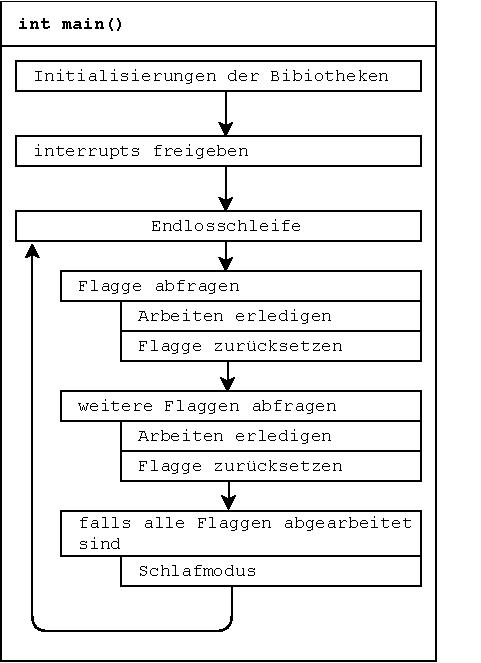
\includegraphics{main_diagram.pdf}
    \caption{Der Grundablauf schematisch dargestellt}
    \label{img:grundablauf}
\end{figure}
\newline
Der Grundablauf ist in Abbilung \ref{img:grundablauf} zusehen. Es wird zuerst der Mikrorechner und alle benötigten Systeme Initialisiert und dann in den interrupt-gesteuerten Betrieb Übergegangen. Der Prozessor wird also in den Schlaf- bzw. Low-Power-Modus versetzt und reagiert ab sofort nur noch auf auftretende interrupts (engl. Unterbrechungen). Die aufgerufene interrupt service routine (ISR) soll möglichst schnell abgearbeitet werden, also wird meist lediglich das interrupt ausgewertet und dann eine entsprechende Flagge gesetzt. Dann wird der Schlafmodus verlassen und die ISR beendet. Durch das Verlassen des Schlafmodus werden nun in der main()-Funktion die nächsten Befehle ausgeführt. Hier werden nun die Flaggen abgefragt und die entsprechenden Arbeiten erledigt. Sobald alle Flaggen abgefragt und abgearbeitet sind, wird der Prozessor wieder in den Ruhemodus versetzt. Diese Abarbeitung in der main()-Funktion hat den großen Vorteil, dass lang andauernde Arbeiten (z.B. Ansteuerung des Displays mit Wartezeiten) durch interrupts unterbrochen und diese ausgewertet werden können, ohne das auf erst die lange andauernden Anweisungen gewartet werden muss. Diese Blockierung der schnell abzuarbeitenden ISRs passiert, würden alle Aufgaben in ISRs passieren und nicht in der main()-Funktion. Zeitkritische Aufgaben z.B. Tastendrücke oder Töne könnten nicht richtig oder zeitnah ausgelesen bzw. ausgegeben werden.

\subsection{Modulstruktur}
Die Programmierung des Mikrorechners erfolgte in Teilmodulen, die grob den verschiedenen Teilen des Projekts entsprechen. Diese Teilmodule des Projekts wurden erst für sich entwickelt und sobald ein passabler Grad der Implementierung erreicht wurde in das Gesamtprojekt eingebunden und im Verbund getestet. Das Projekt wurde in folgende Module zerlegt:
\begin{itemize}
	\item Display-Ansteurung (\textsl{lcd.h})
	\item Eingaben, also Taster und Drehgeber (\textsl{input.h})
	\item Uhrzeit (\textsl{clock.h})
	\item Alarm (\textsl{alarm.h})
	\item Tonerzeugung (\textsl{tone.h})
	\item Melodien (\textsl{melodies.h})
	\item LED-Matrix (\textsl{ledmatrix.h})
	\item Menüführung (\textsl{menu.h})
\end{itemize}
Hauptfluss des Programms passiert natürlich grundsätzlich in der \textsl{main.c} mit der \textsl{main}-Funktion, aber die Zustände und Zustandsänderungen werden durch das Menü also die \textsl{Menü}-Bibliothek geregelt, die alle anderen Bibliotheken einbindet und zum gesamten Programm verbindet.

\section{Module}
Hier werden die Module genauer in ihrem Aufbau und ihrer Struktur beschrieben. Die Modulnamen für die tatsächlichen Dateien sind in Klammern angegeben und umfassen die entsprechende *.h und *.c Dateien.

\subsection{\source{main.c}}
Die \source{main.c}-Datei ist der Einstiegspunkt des Programms und enthält die Funktion \source{int main()}. Es werden alle unserer Bibliotheken inkludiert, damit diese gleich zu Beginn durch ihre Initialisierungsfunktionen initialisiert werden können. Danach werden interrupts freigegeben und das Programm startet die Hauptschleife und damit den interrupt-basierten Ablauf, wie im Abschnitt Grundstruktur und in der Abbildung \ref{img:grundablauf} erläutert.
\newline
Es werden außerdem die zwei ISRs der beiden Timer A und Timer B implementiert, da diese teilweise von mehreren Bibliotheken benötigt werden und deswegen von dieser zentralen Stelle diese Bibliotheken aufrufen. Dies wird für die Uhrzeit-, Ton- und LED-Matrix-Bibliotheken getan.
\newline
Es werden außer den ISRs noch ähnliche Funktionen definiert, die durch Bibliotheken für bestimmte Ereignisse aufgerufen werden. Dies sind \source{void new\_minute()}, das von der Uhrzeit-Bibliothek aufgerufen wird, sobald eine neue Minute angebrochen ist und die Funktion \source{void alarm\_ring()}, die signalisiert, dass ein Alarm ausgelöst worden ist und nun klingeln soll. Diese Funktionen wurden in die \source{main.c} Datei verlegt, da diese Ereignisse Veränderungen in mehreren Bibliotheken auslösen: \source{void new\_minute()} bedeutet, dass die Alarme überprüft werden müssen und die LED-Matrix aktualisiert werden muss;
\source{void alarm\_ring()} bedeutet, dass das Menü in den Alarm-Modus übergehen muss und die Melodie des entsprechenden Alarms gestartet wird.

